This section analyses the effects of independent Q-learning, as well as different parameter settings for this learning method.
\subsubsection{1 predator vs. 1 prey}
To start off, a test was run to see if the new environment behaves as expected. Not much has changed, except allowing multiple predators to be initialized, different functions for Q-learning and policies (they need to be dynamic and change with the number of agents) and the caveat that the prey has to trip during $20\%$ of its actions.

\begin{center}
	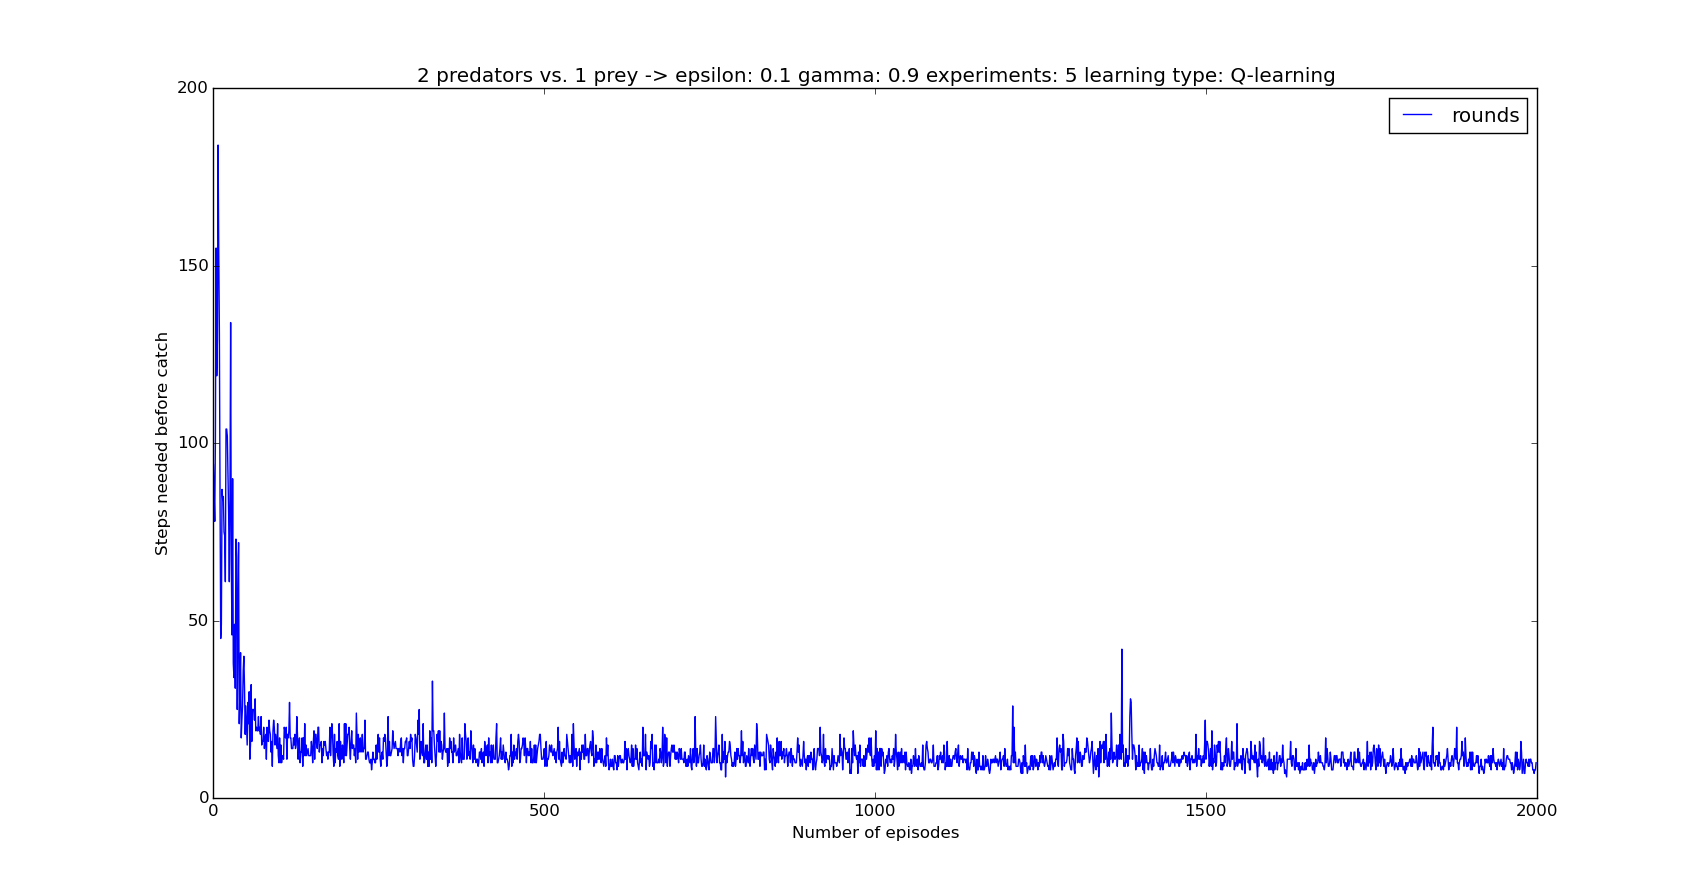
\includegraphics[scale=0.3]{1_predator_1_prey_q_learning}
	\captionof{figure}{Independent Q-learning: 1 predator versus 1 prey}
	\label{graph:1vs1}
\end{center}

As the graph in figure \ref{graph:1vs1} shows, the predator learns how to catch the prey more quickly after each time step. However, in the previous implementation, the number of time steps it took the predator to catch the prey became more stable. Though the number of time steps needed to catch the prey drops significantly (apparently, the $20\%$ trip rate more than offsets the intelligence of the prey), there is more variance than before. Also, the algorithm learns more quickly than before. As the state space grows exponentially with every added predator,  the state space was encoded to reduce the amount of possible states and is now of size $11^2$. Therefore, after the predator has spent enough time learning, each greedily chosen action is always in the direction of the prey. This leads to catching the prey quicker than before as there is a much smaller state space to be explored.

\subsubsection{2 predators versus 1 prey}
In this case, there are two predators hunting one prey. The state space is now larger than before ($11^4$ states) and leads to slower computations. Tests have shown that the amount of rounds it takes for any of the predators to catch the prey vary significantly, but more importantly, cannot be informatively represented in a graph. Therefore, the cumulative wins and losses for the predators have been graphed, rather than the amount of rounds it takes the predators to catch the prey. Unsurprisingly,  as shown in figure \ref{graph:2vs1}, the graph for wins becomes steeper, and the graph for losses becomes flat after learning. This indicates that the predators are winning more and losing less. Moreover, the numbers of rounds it takes for the predators to catch the prey improves over time. These numbers have been tracked and logged in table \ref{table:2vs1} below.

\begin{center}
	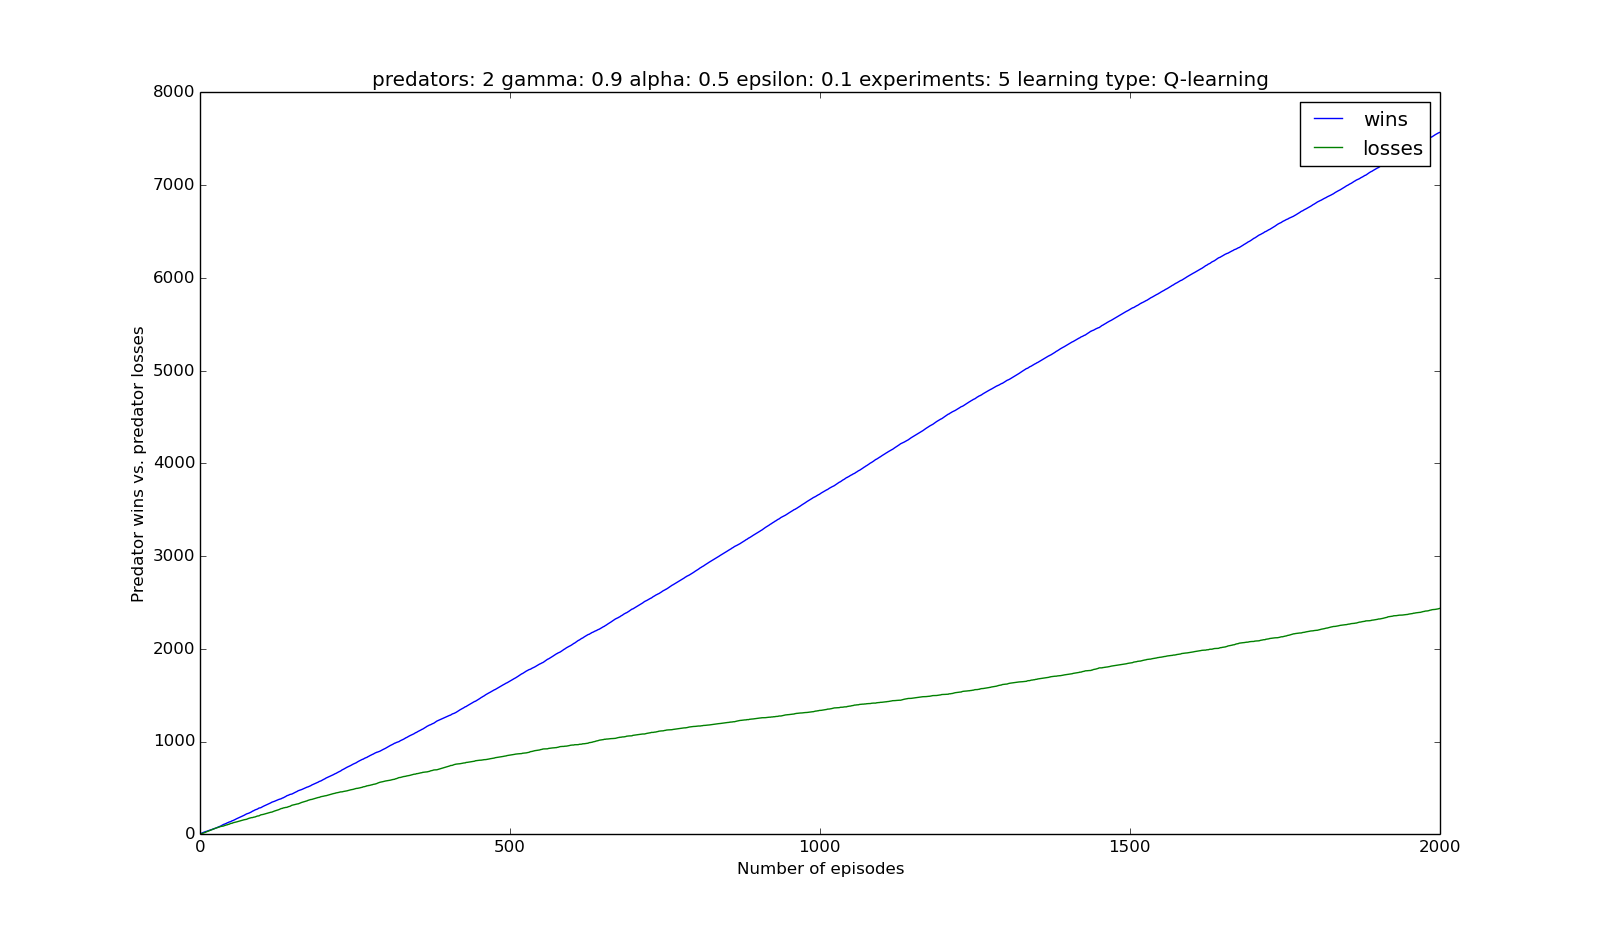
\includegraphics[scale=0.3]{2_predators_q_learning}
	\captionof{figure}{Independent Q-learning: 2 predators vs. 1 prey}
	\label{graph:2vs1}
\end{center}

%The graph shows that the predators learn to cooperate and catch the prey. This number increases, as the number of predator losses increases more slowly over time, while the number of predator wins increases more quickly over time. As this is counted cumulatively, it can be expected that the number of wins by the prey will become almost steady. 

It is expected that, in the end, the predators will win almost each game. As the policies of the predators and the prey are still exploratory, it is possible for two predators to bump into one another and lose the game.

The table \ref{table:2vs1} shows the average number of rounds the predators need to catch the prey.

\begin{table}[H]
\begin{center}
\begin{tabular}{| l | l | l | l | l |}
\hline
 & \parbox{2cm}{\textbf{Avg wins \\ (first 100)}} & \parbox{2cm}{\textbf{Avg losses \\ (first 100)}} & \parbox{2cm}{\textbf{Avg wins \\ (last 100)}} & \parbox{2cm}{\textbf{Avg losses \\ (last 100)}} \\
\hline
\textbf{Predators} & 58 & 42 & 76 & 23 \\
\hline
\end{tabular}
\caption{Average number of rounds two predators need to catch one prey}
\label{table:2vs1}
\end{center}
\end{table}

As the table shows, the predators learn to catch the prey quicker over time.

\subsubsection{3 predators versus 1 prey}
With four agents on the grid, the implementation became very slow. It was possible to run the implementation, but as it is very slow, the parameter changes have not been tested. However, figure \ref{graph:3vs1} shows the results of running three predators versus one prey. Due to time constraints and the amount of time it takes for the algorithm to calculate the all the states, this was for 1000 episodes. Contrary to the other testing approaches, this test was run once and so not averaged over several experiments.

\begin{center}
	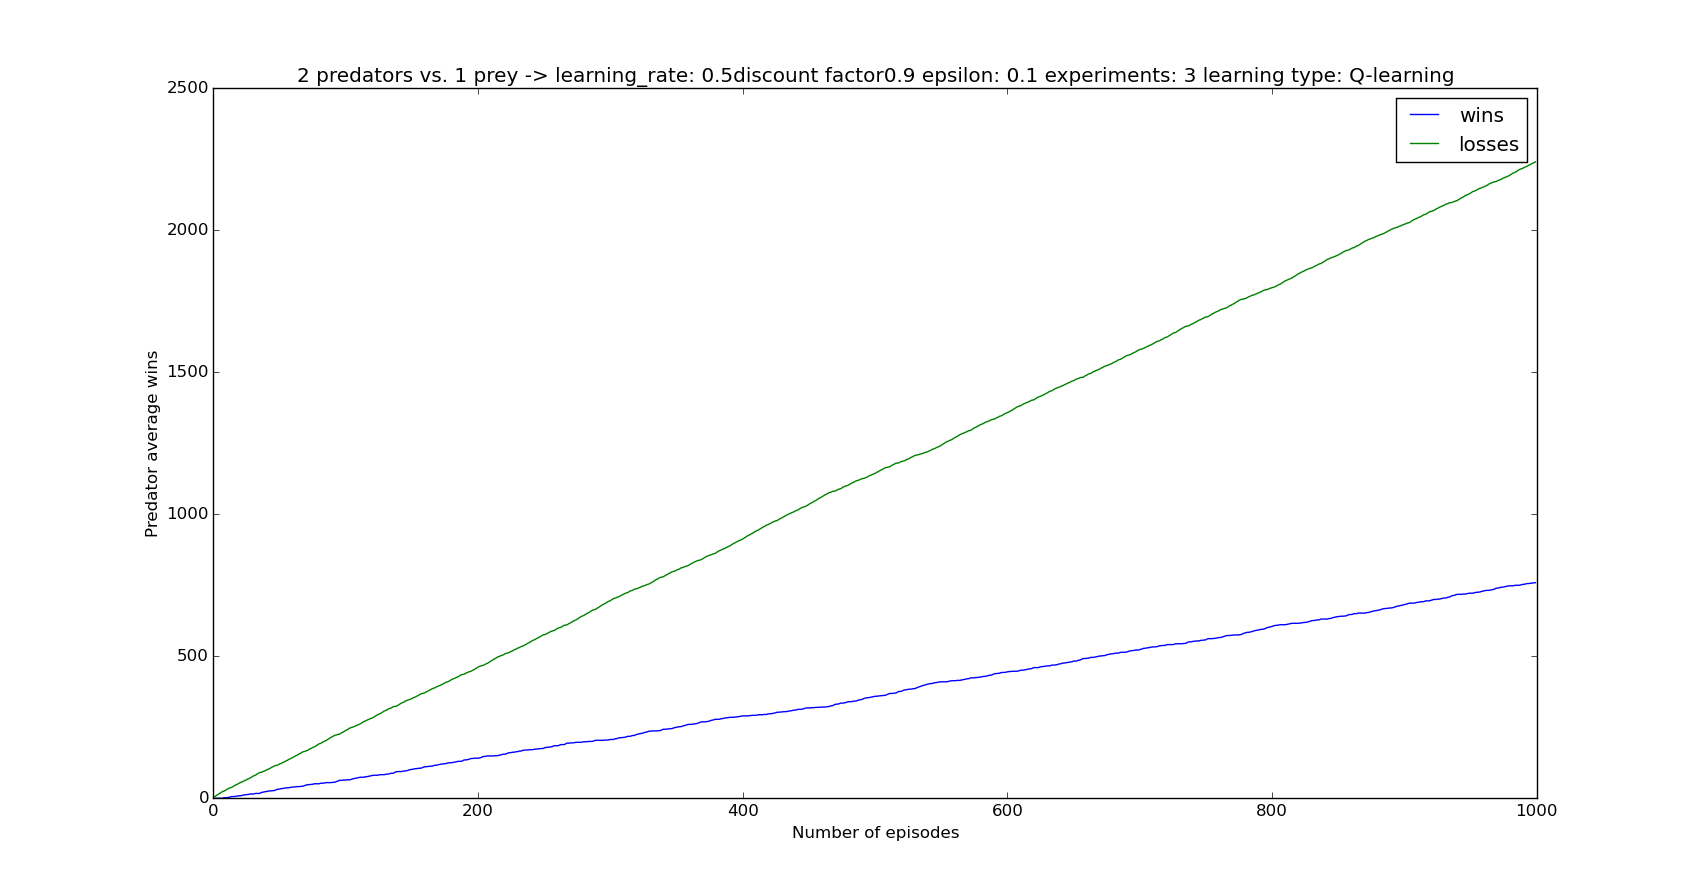
\includegraphics[scale=0.3]{3_predators_3_ex_1000_runs_q-learning}
	\captionof{figure}{Independent Q-learning: 3 predators vs. 1 prey}
	\label{graph:3vs1}
\end{center}


\newcommand{\labelerrorfootnote}{\footnote{Due to a labeling error during test execution, the title which appears on the figure itself does not match the one under the figure. The one under the figure is the correct one and the figure does reflect the results for 3 predators vs. 1 prey.}}

Figure \ref{graph:3vs1} shows that the predators lose the game a lot.\labelerrorfootnote \: This is interesting as it is expected of the predators to learn not to bump into one another. However, the grid is both toroidal as well as small and the prey learns. It is possible that the prey learning, combined with a small, toroidal grid, leads to the predators bumping into one another. Perhaps the prey learns to trick the predators into bumping into one another. Therefore, it is interesting to see what happens if the prey learns slower than the predators. By making the prey learn slower, theoretically it is possible for the predators to learn not to bump into one another and catch the prey. In order to simulate this, the predators learn as stated in default, but the prey learns with a learning rate of 0.01. These results are shown in figure \ref{graph:3vs1slowprey}.

\begin{center}
	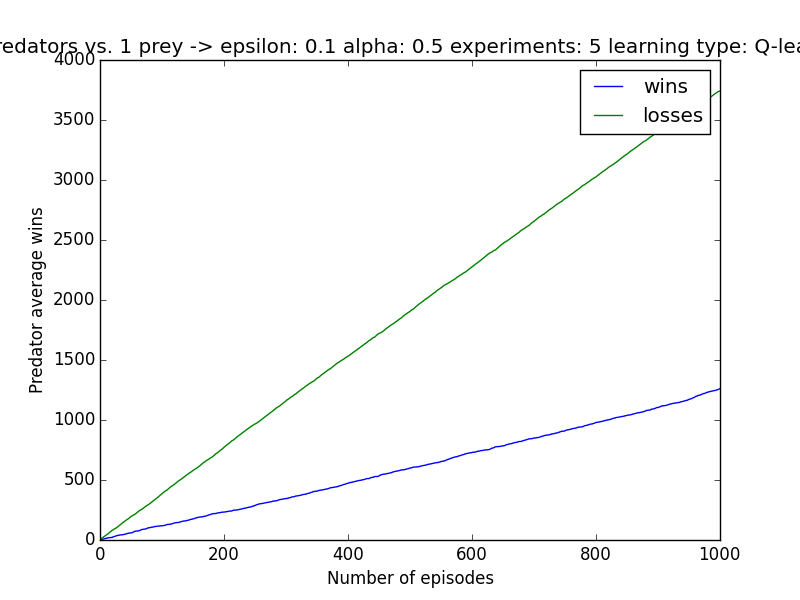
\includegraphics[scale=0.3]{smaller_learning_rate_prey}
	\captionof{figure}{Independent Q-learning: 3 predators vs. 1 prey, slow learning prey}
	\label{graph:3vs1slowprey}
\end{center}

Table \ref{table:3vs1} shows the results of the first- and last 100 wins and losses of the predators.

\begin{table}[H]
\begin{center}
\begin{tabular}{| l | l | l | l | l |}
\hline
 & \parbox{2cm}{\textbf{Avg wins \\ (first 100)}} & \parbox{2cm}{\textbf{Avg losses \\ (first 100)}} & \parbox{2cm}{\textbf{Avg wins \\ (last 100)}} & \parbox{2cm}{\textbf{Avg losses \\ (last 100)}} \\
\hline
\textbf{Default learning rate} & 21 & 78 & 25 & 73 \\
\hline
\textbf{Low learning rate} & 23 & 76 & 31 & 68 \\
\hline
\end{tabular}
\caption{Average number of wins and losses by the predators with varying learning rates}
\label{table:3vs1}
\end{center}
\end{table}

The results in table \ref{table:3vs1} show that the predators do learn to catch the prey. When the prey learns slower, the predators manage to catch the prey more often in the same amount of time. Therefore, it can be concluded that the algorithm does learn the predators to cooperate and catch the prey. This just takes many episodes.

\subsubsection{4 predators versus 1 prey}
Though it is implemented for four predators and one prey to be placed on the grid, this leads to implementations freezing. It is therefore conclusive to state that the program has become intractable. This could be solved by using function approximation, for example using Kanerva coding \cite{wu2009function}, where a number of \textit{prototype} state-action pairs are selected, to be used for storing Q-values for similar state-action pairs. Another possible solution is to have the predators learn \textit{together}, meaning they share a Q-value grid and learn simultaneously. However, this is not truly independent Q-learning. 

\subsubsection{Parameter settings}
It is interesting to see what happens when the parameters of the learning methods change. As the effects of parameter settings have been researched in a 1 vs. 1 scenario, it is interesting to see what is different when there are more agents on the grid. Also, as all agents now learn, the effects of these learning methods should change.

\subsubsection{Learning rate}
First, the effect of the learning rate is researched. As the learning rate determines to what extent the newly acquired information will override the old information, it is interesting to see what happens.

\begin{center}
	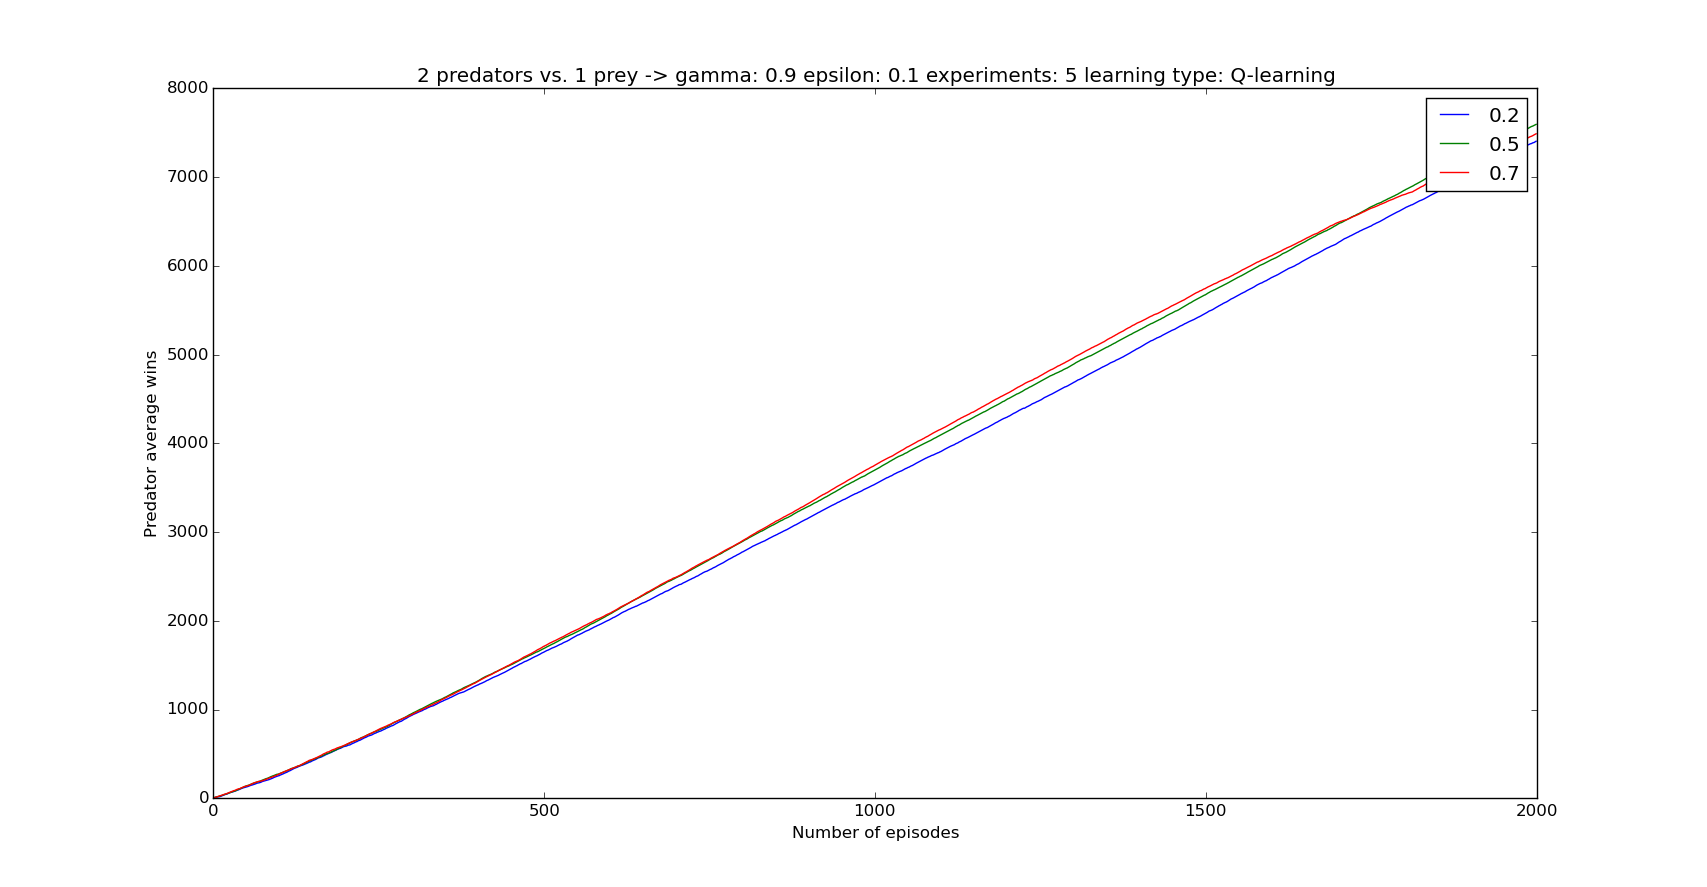
\includegraphics[scale=0.3]{2_predators_learning_rate_q_learning}
	\captionof{figure}{Independent Q-learning: 2 predators vs. 1 prey, learning rate}
	\label{graph:learningrate}
\end{center}

Figure \ref{graph:learningrate} shows that a low learning rate yields worst results. For a long time, a high learning rate yields good results, however, in the end a learning rate of 0.5 yields best results. This shows that for a long time, a lot of recent information is interesting.  Later on, however, an even balance of new and old information leads to more wins for the predator. 

\begin{table}[H]
\begin{center}
\begin{tabular}{| l | l | l | l | l |}
\hline
\parbox{2cm}{\textbf{Learning rate}} & \parbox{2cm}{\textbf{Avg wins \\ (first 100)}} & \parbox{2cm}{\textbf{Avg losses \\ (first 100)}} & \parbox{2cm}{\textbf{Avg wins \\ (last 100)}} & \parbox{2cm}{\textbf{Avg losses \\ (last 100)}} \\
\hline
\textbf{0.2} & 50 & 49 & 74 & 24 \\
\hline
\textbf{0.5} & 54 & 45 & 72 & 27 \\
\hline
\textbf{0.7} & 54 & 45 & 63 & 35 \\
\hline
\end{tabular}
\caption{Average number of wins and losses by the predators with varying learning rates}
\label{table:learningrate}
\end{center}
\end{table}

Table \ref{table:learningrate} shows that the lowest learning rate shows better and better results over time. This shows that in the beginning, a lot must be learned. As the game progresses, a low learning rate yields better results. This could indicate that the predators as well as the prey become predictable and so less new information has to be learned. As minimax Q-learning contains a decay in learning, perhaps this is the reason why.\red{THIS IS INDEED STRANGE!!!! }  %this is strange.  


\subsubsection{Discount factor}
The discount factor determines the importance of future rewards. In the previous assignment, when only one predator was learning, a high discount factor yielded best results. This means that the future reward was most important. Only the goal state yielded a reward, making reaching the goal state very important. Currently, there are two terminal states: the win state and the lose state. It is interesting to see what effect the negative rewards have on the importance of the immediate reward.

\begin{center}
	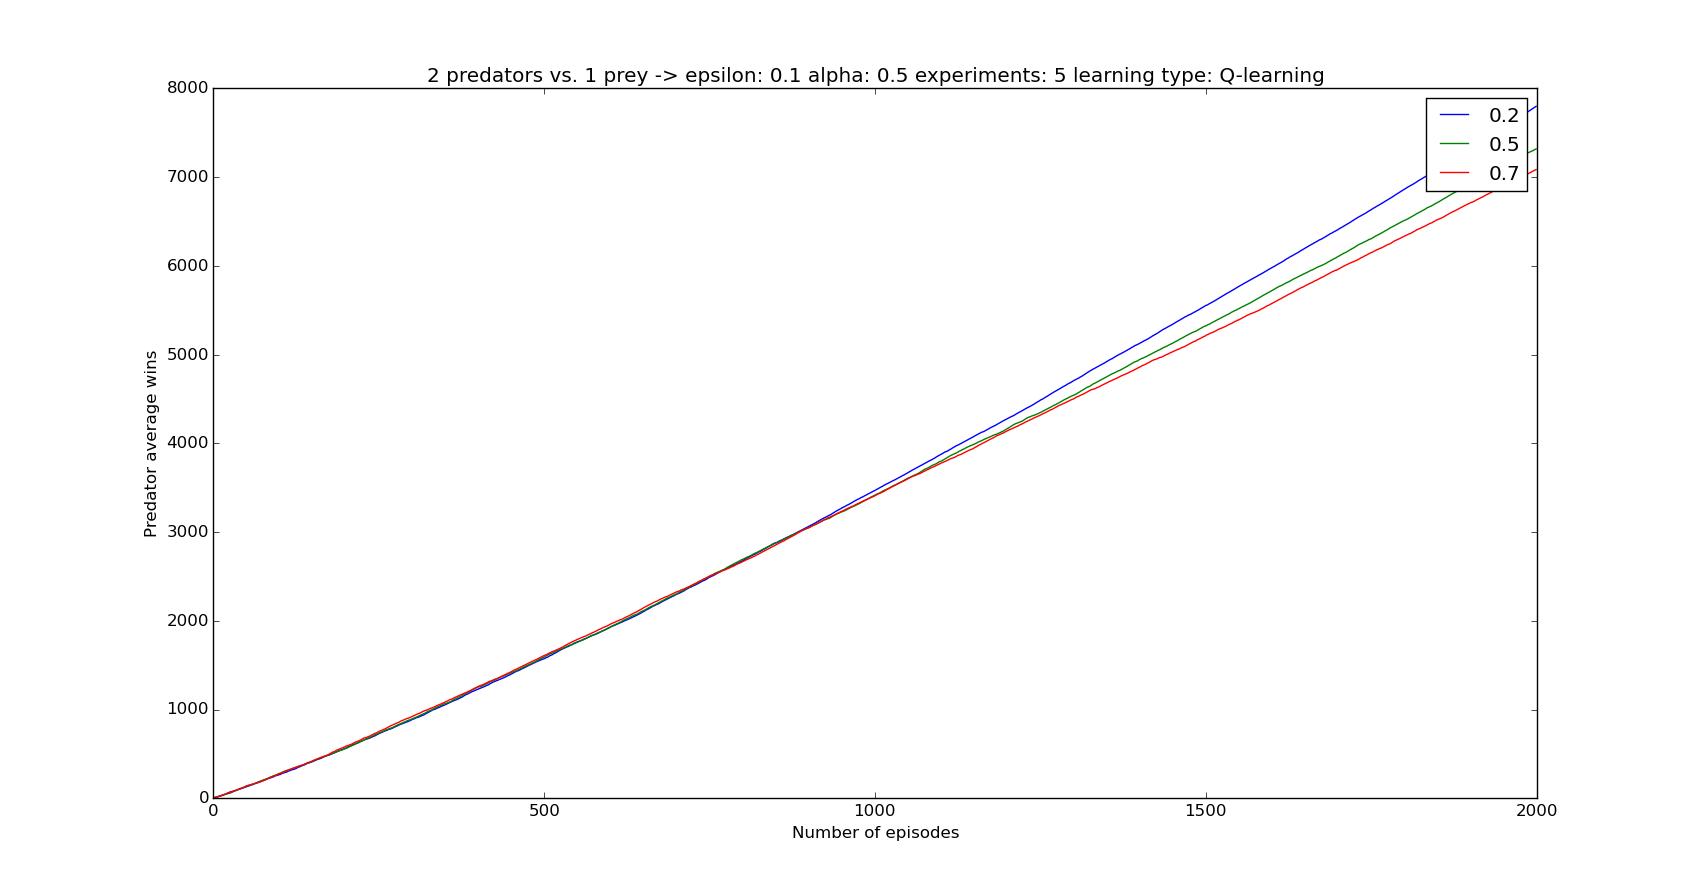
\includegraphics[scale=0.3]{2_predators_discount_factor_q_learning}
	\captionof{figure}{Independent Q-learning: 2 predators vs. 1 prey, discount factor}
	\label{graph:discountfactor}
\end{center}

Figure \ref{graph:discountfactor} shows that for a long time, it does not matter how important the future reward is. However, eventually the graph shows that a low discount factor yields best results. This might be caused by the fact that the predators will receive a negative reward when running into another predator. In order to avoid this, winning (or not losing) immediately is more important than expected future rewards.

\begin{table}[H]
\begin{center}
\begin{tabular}{| l | l | l | l | l |}
\hline
\parbox{2cm}{\textbf{Discount factor}} & \parbox{2cm}{\textbf{Avg wins \\ (first 100)}} & \parbox{2cm}{\textbf{Avg losses \\ (first 100)}} & \parbox{2cm}{\textbf{Avg wins \\ (last 100)}} & \parbox{2cm}{\textbf{Avg losses \\ (last 100)}} \\
\hline
\textbf{0.2} & 52 & 47 & 98 & 4 \\
\hline
\textbf{0.5} & 55 & 44 & 78 & 21 \\
\hline
\textbf{0.7} & 55 & 45 & 74 & 24 \\
\hline
\end{tabular}
\caption{Average number of predator wins and losses for varying discount factors}
\label{table:discountfactor}
\end{center}
\end{table}

Table \ref{table:discountfactor} shows that the discount factor has a huge impact on the success of the predators. By making sure that the predators do not run into each other, the game is not lost as often.

\subsubsection{$\epsilon$-greedy action selection}
In the current implementation, $\epsilon$-greedy action selection was used to find actions for the agents. For this action-selection mechanism, $\epsilon$ determines the percentage of greedy versus exploratory actions. An $\epsilon$ value of 0 selects only greedy actions. The closer this value is to 1, the more exploring actions are selected. The following figure \ref{graph:greedy} shows the results of this test.

\begin{center}
	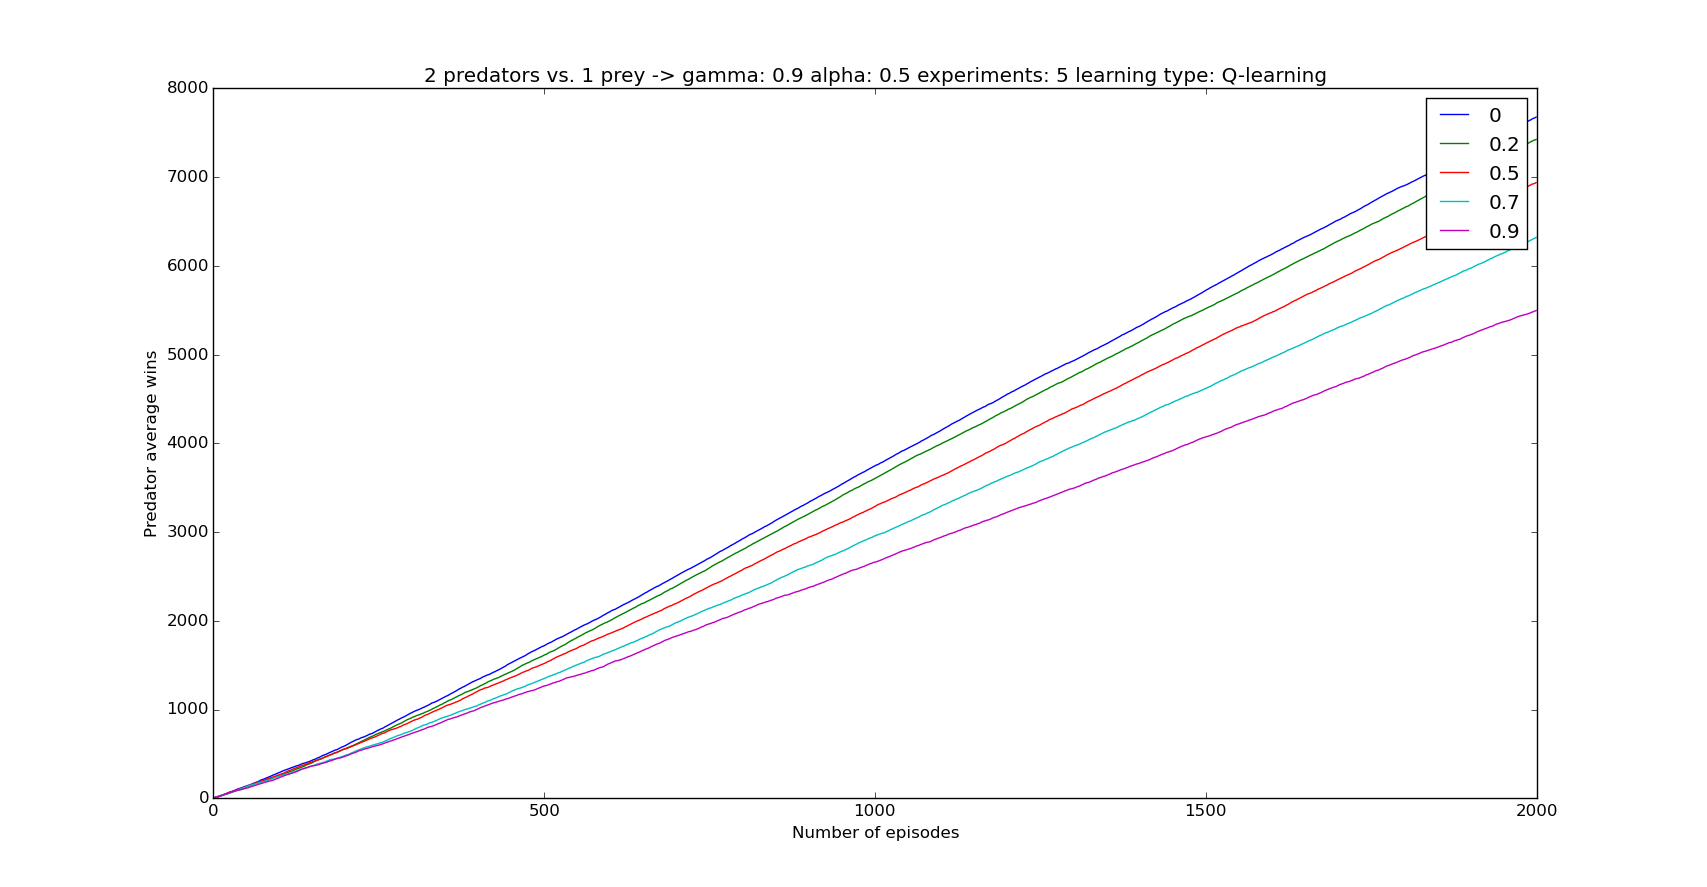
\includegraphics[scale=0.3]{2_predators_epsilon_q_learning}
	\captionof{figure}{Independent Q-learning: 2 predators vs. 1 prey, $\epsilon$-greedy action selection}
	\label{graph:greedy}
\end{center}

Figure \ref{graph:greedy} shows that greedy action selection yields best results. This is possible, as all predators are initialized at the corners of the grid, starting out with equal distance to the prey. As the prey moves, it will be closer to one predator. Therefore, after learning and without exploration, the prey will be caught by one predator (as it tries to minimize the distance between the prey and itself). As a greedy action, in this case, leads to moving in the direction of the highest Q-value, it is still possible for the predators to bump into each other. However, it seems as if the prey is most often caught before this happens leading to wins for the predators.

\begin{table}[H]
\begin{center}
\begin{tabular}{| l | l | l | l | l |}
\hline
\parbox{2cm}{\textbf{$\epsilon$-rate}} & \parbox{2cm}{\textbf{Avg wins \\ (first 100)}} & \parbox{2cm}{\textbf{Avg losses \\ (first 100)}} & \parbox{2cm}{\textbf{Avg wins \\ (last 100)}} & \parbox{2cm}{\textbf{Avg losses \\ (last 100)}} \\
\hline
\textbf{0} & 55 & 44 & 76 & 22 \\
\hline
\textbf{0.2} & 54 & 45 & 77 & 21 \\
\hline
\textbf{0.5} & 49 & 50 & 72 & 27 \\
\hline
\textbf{0.7} & 48 & 51 & 66 & 32 \\
\hline
\textbf{0.9} & 50 & 59 & 55 & 44 \\
\hline
\end{tabular}
\caption{Average number of wins and losses by the predators with varying $\epsilon$-rates}
\label{table:greedy}
\end{center}
\end{table}

Table \ref{table:greedy} Though, at first, an absolute greedy policy appears to yield the most promising results, a slightly exploratory policy eventually yields the best results. This is not displayed in the graph as the wins are counted cumulatively. Eventually, the results will be best when still exploring sightly.

\subsubsection{Optimal settings}
As the optimal settings have been found ($\gamma$ = 0.2, $\epsilon$ = 0.2, $\alpha$ = 0.5), two predators were unleashed against the predator. In order to maximize the result of the predators, the learning rate of the prey was also reduced to a minimum of 0.01. This lead to the results displayed in figure \ref{graph:optimal_q_graph} and table \ref{table:optimal_q_table}. However, due to time constraints, this test was run once. These results were not averaged over several experiments\footnote{As one may have noticed, the graph states that this experiment was run for two predators. This was not changed before running the test. However, these results are indeed of three predators versus one prey.}.

\begin{center}
	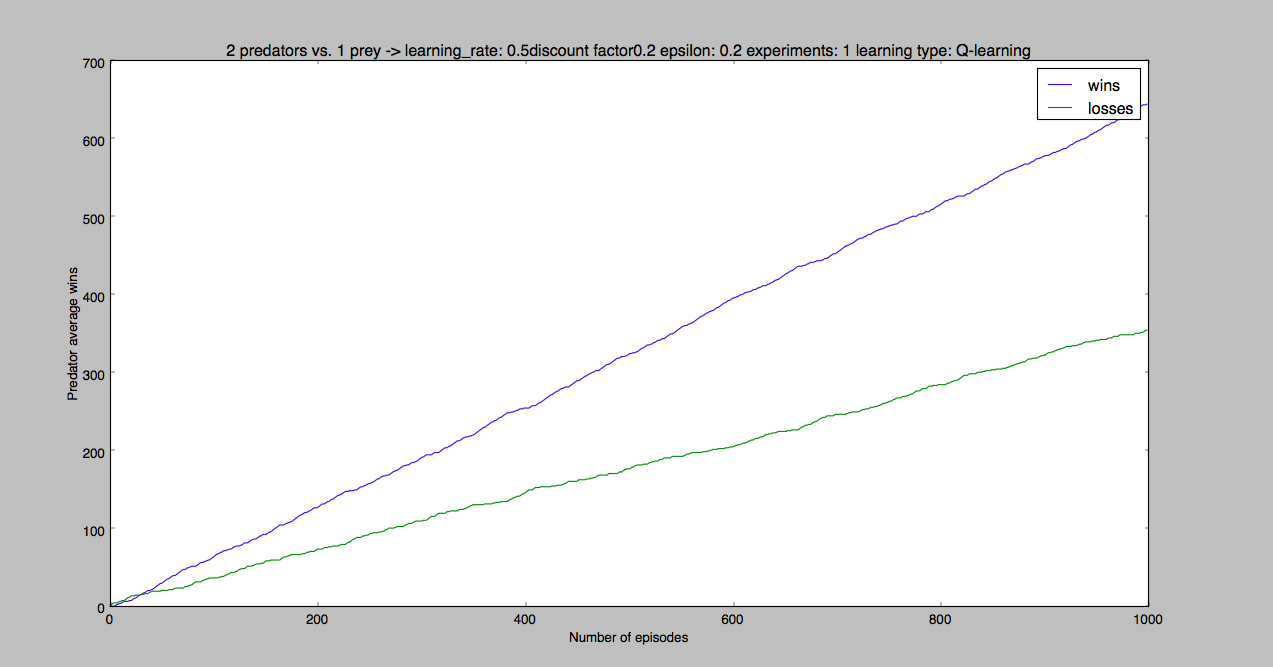
\includegraphics[scale=0.3]{q_learning_optimal_1000times5}
	\captionof{figure}{Independent Q-learning: 3 predators vs. 1 prey, optimal settings}
	\label{graph:optimal_q_graph}
\end{center}

The graph shows a significant difference with the previous test of three predators versus one prey. 

\begin{table}[H]
\begin{center}
\begin{tabular}{| l | l | l | l | l |}
\hline
\parbox{2cm}{\textbf{$\epsilon$-rate}} & \parbox{2cm}{\textbf{Avg wins \\ (first 100)}} & \parbox{2cm}{\textbf{Avg losses \\ (first 100)}} & \parbox{2cm}{\textbf{Avg wins \\ (last 100)}} & \parbox{2cm}{\textbf{Avg losses \\ (last 100)}} \\
\hline
\textbf{Optimal} & 63 & 37 & 67 & 32 \\
\hline
\end{tabular}
\caption{Average number of wins and losses by the predators with optimal values}
\label{table:optimal_q_table}
\end{center}
\end{table}

Table \ref{table:optimal_q_table} shows that the predators are winning in most episodes and this number has increased near the end of the experiment. This shows how powerful choosing the correct parameters is when implementing an algorithm.
